% Latex Style for CMP PGR DAY 2009.
%
% Revision 1.0
% Feb. 12 2009.
%
% Barry-John Theobald, University of East Anglia, Norwich, UK

\documentclass{cmppgr}

\usepackage[pdftex]{graphicx}
\graphicspath{{figures/}}

\title{Algorithm X is better than Y when classify Z data 2017 --- Norwich, UK}
\name{Luke M. Garrigan}
\institution{
	Machine Learning, University of East Anglia, UK
}
\email{l.garrigan@uea.ac.uk}



\begin{document}
\maketitle

\begin{abstract}

This is the paper layout specification and template definition for the 2009 CMP Research Day. You should submit either an 8 or 4 page paper according to your choice made the end of August. Following your abstract, you should include a list of keywords relating to the subject in your paper --- these should appear as a comma separated list, as in the examples below. You have to submit it in latex, if you are not tex compliant use this template and get some help!

\end{abstract}

\keywords{Relevant topics, list here, makes searching easier}

\section{Introduction}

This paper template can be found on the CMP website (\texttt{  }), with  the \LaTeX\ source and the style file you should use to generate your paper. To ensure consistency in the presentation of the proceedings, all authors are required to typeset their document using \LaTeX, and use the research day style file, as follows: \texttt{$\backslash$documentclass\{cmppgr\}}. You should be the first author on this paper. You should discuss co-authors with your supervisor. {\bf Do not put anyone down as a co-author without their express permission}, even if this is a reworking of an existing paper. Compile this with pdflatex.

\section{Page layout and style}

This document includes examples of all of the likely environments authors will require in their papers. You are strongly encouraged to compare your document with this reference example. Submissions that do not match the formatting laid out here will be returned to the submitting author for correction.

\subsection{Sections}

Section headings should be centred on the line, be in bold typeface, and only the first letter should be capitalised. Sub-headings are also in bold face, but appear flush left and are typeset in the base font size. Sub-sub-headings appear like sub-headings, except they are in italics and are not boldface. No more than 3 levels of headings are allowed.

\subsection{Headers and Footers}

All headers and footers must be left empty. Your document should not contain page numbers etc. These will be added later.

\subsection{Lists}

Itemised lists can be included in your document, but please check the indentation if you are not using \LaTeX. An example itemized list with the correct formatting should look like the following:
%
\begin{itemize}
\item{First list item.}
\item{Second list item.}
\item{Third list item.}
\end{itemize}
%

\subsubsection{List Depth}

Please try not to use hierarchical lists, these look cluttered in two-column format. Keep lists to a single level of depth.

\subsection{Figures}

All figures must be centred on the column (or page, if the figure spans both columns). A figure caption should follow the figure and be formatted like the example in Figure~\ref{fig:columnfigure}.

\begin{figure}[h]
\centering
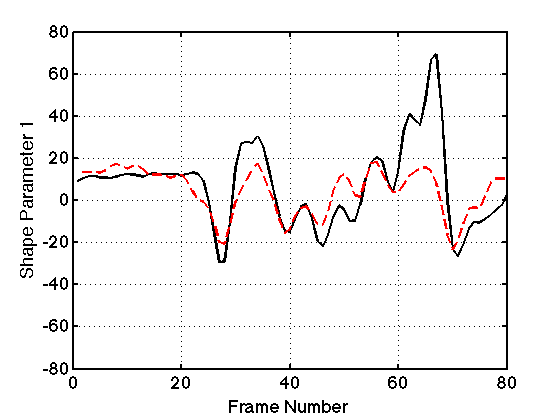
\includegraphics[scale=0.4]{sparam_1_errors}
\caption{An example of a figure centred on a single column. The figure is not centred automatically. To centre the figure, use \texttt{$\backslash$centering} within the \texttt{figure} environment.}
\label{fig:columnfigure}
\end{figure}

Figures spanning multiple columns should appear either at the top or the bottom of the page. You can use the $\backslash$figure* command to span a figure across both columns. An example is shown in Figure~\ref{fig:pagefigure}.

\begin{figure*}[tb]
\centering
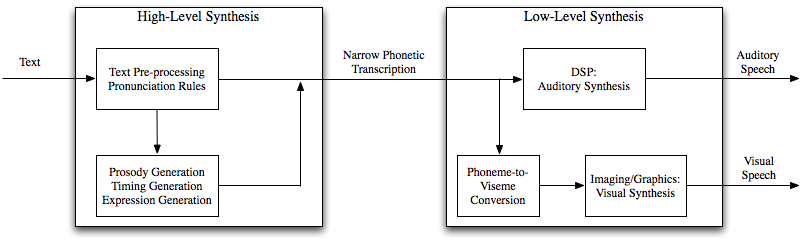
\includegraphics[scale=0.5]{AVTTS-Overview}
\caption{An example of a figure spanning both columns and centred on a page. Again, the figure is not centred automatically.}
\label{fig:pagefigure}
\end{figure*}

Figures should preferably be line drawings. The proceedings will not be produced in colour, so please do not rely on colour to distinguish between curves on a graphs, etc. You should check to ensure the figures print well on a good quality printer, and that there are no issues when colour figures are printed in grey-scale.

Before including any figures in your document you should ensure you have the necessary copyright permission.

\subsection{Tables}

Tables should be centred on a column if possible. There is no strict requirement on the style as this will largely depend on the content to be displayed. An example table is shown in Table~\ref{tab:example}, but this is provided for illustrative purposes only.

\begin{table}[h]
\centering
\caption{An example table.}
\begin{tabular}{|c|c|}
\hline
Trial & Score \\\hline\hline
1 & 10 \\
2 & 12 \\
3 & 11 \\
4 & 9 \\
5 & 11 \\
6 & 10 \\\hline
\end{tabular}
\label{tab:example}
\end{table}

Note, for tables the caption should be above the table, as shown in Table~\ref{tab:example}.

\subsection{Equations}

Equations should appear on a separate line, they should be centred and they should be numbered. Some examples are:
%
\begin{equation}
y = mx + c,
\label{eqn:line}
\end{equation}
%
which obviously is the equation of a straight-line of gradient $m$ and intersecting the vertical axis at $c$. Another famous equation with $m$ and $c$ is
%
\begin{equation}
E = mc^2.
\label{eqn:einstein}
\end{equation}

\subsection{Fonts}

You should use 9 point Times or Times Roman for the main text. All fonts should be embedded in the final PDF document.

\subsection{Hyperlinks}

Hyperlinks should be written in full, e.g., \texttt{http://www.cmp.uea.ac.uk}, and must be coloured black. For ease of readability, authors are advised to use a different font family from the main text.

\subsection{Supplementary Material}

Authors may submit supplementary material with their paper. However, this should not be included in place of a technical description of your work. Reviewers are not obliged to watch video sequences, and your submission will be reviewed on the strength of the paper only. If you are submitting a multimedia file, please use widely accepted formats/codecs. The conference proceedings will not include media players.

\section{Conclusions}

The page limit is 4--6 pages. Please, please use \LaTeX\ to typeset your document. This will minimise any formatting headaches!

\subsection{References}

You must reference any papers you have had accepted or are under review here. Example references~\cite{massaro98:perceiving}, audio-visual speech synthesis~\cite{theobald04:specomm,theobald08:lips}, and audio-visual speech recognition~\cite{cox08:avsp,matthews2002:extraction}.

See the references section for the formatting of the references from different sources (conferences, journals, and books). The formatting of references follows the standard IEEE format, \LaTeX\ users should download the \texttt{IEEEtran} bibliography format. References should be listed in order of citation.

\bibliographystyle{IEEEtran}
\bibliography{sample_bib.bib}

\end{document}
